\subsection{Filtro bayesiano de spam}

\subsubsection{Descrição do problema e hipóteses probabilísticas}

A filtragem de mensagens indesejadas é um problema clássico de classificação
probabilística em Computação. Cada mensagem de correio eletrônico deve ser
atribuída a uma de duas classes, spam, a mensagem indesejada, ou não spam, a
mensagem legítima. O classificador observa apenas as palavras presentes na
mensagem e precisa decidir, sob incerteza, a qual classe ela pertence. O
classificador bayesiano ingênuo é uma das abordagens mais usadas para essa
tarefa \cite{metsis2006spam}.

O modelo parte de um vocabulário fixo de $d$ palavras escolhidas de antemão,
como \textit{grátis}, \textit{promoção} e \textit{reunião}. Cada mensagem é então
representada por um vetor binário $x = (x_1, \ldots, x_d)$, em que $x_j = 1$ indica
que a palavra de índice $j$ do vocabulário aparece na mensagem e $x_j = 0$ indica
que ela não aparece. O método assume duas hipóteses probabilísticas, a primeira é
que cada classe tem uma probabilidade a priori de ocorrência, $P(S)$ para spam e
$P(\bar{S})$ para não spam. A segunda, é a hipótese
ingênua de independência condicional, segundo a qual a presença de cada palavra
é independente das demais quando a classe é conhecida \cite{sahami1998bayesian}.
Essa suposição raramente vale no texto real, já que certas palavras tendem a
ocorrer juntas, mas simplifica a modelagem e produz classificadores eficazes na
prática \cite{metsis2006spam}.

\subsubsection{Modelagem probabilística}

A decisão tem como base o Teorema de Bayes \cite{chan2021probability}. Dada a
mensagem $x$, a probabilidade a posteriori de a mensagem ser spam é obtida pela
Equação~\ref{eq:bayes_spam}.

\begin{equation}
	P(S \mid x) = \frac{P(x \mid S)\, P(S)}{P(x \mid S)\, P(S) + P(x \mid \bar{S})\, P(\bar{S})}
	\label{eq:bayes_spam}
\end{equation}

Na Equação~\ref{eq:bayes_spam}, $P(x \mid S)$ é a verossimilhança da mensagem sob
a classe spam. Sob a hipótese de independência condicional, essa verossimilhança
é o produto das probabilidades de cada palavra, conforme a
Equação~\ref{eq:nb_verossimilhanca}, em que $\theta_{jc} = P(x_j = 1 \mid c)$ é a
probabilidade de a palavra $j$ aparecer em uma mensagem da classe $c$.

\begin{equation}
	P(x \mid c) = \prod_{j=1}^{d} \theta_{jc}^{\,x_j} \, (1 - \theta_{jc})^{\,1 - x_j},
	\qquad c \in \{S, \bar{S}\}
	\label{eq:nb_verossimilhanca}
\end{equation}

A mensagem é classificada como spam quando $P(S \mid x) > 0{,}5$. Como a
verossimilhança da Equação~\ref{eq:nb_verossimilhanca} é um produto sobre as
palavras, a probabilidade a posteriori pode ser atualizada a cada palavra
observada.

As probabilidades $\theta_{jc}$ não são conhecidas e precisam ser estimadas a
partir de um conjunto de treinamento. A estimativa adotada é a frequência
relativa da Equação~\ref{eq:theta_freq}, em que $n_{jc}$ é o número de mensagens
da classe $c$ que contêm a palavra $j$ e $n_c$ é o total de mensagens da classe
$c$. É comum corrigir essa estimativa com a suavização de Laplace, que soma
contagens fixas ao numerador e ao denominador para evitar valores iguais a zero,
os quais anulariam o produto da Equação~\ref{eq:nb_verossimilhanca}. Neste
experimento toda palavra aparece em ambas as classes, de modo que
nenhuma estimativa é zero e a frequência relativa é usada diretamente.

\begin{equation}
	\hat{\theta}_{jc} = \frac{n_{jc}}{n_c}
	\label{eq:theta_freq}
\end{equation}

\subsubsection{Implementação em R}

Para validar o método, os dados foram gerados de forma controlada. As
probabilidades verdadeiras, tanto a priori de cada classe quanto a probabilidade
de cada palavra em cada classe, foram escolhidas de antemão para representar um
cenário plausível e servem de referência conhecida. A partir delas, cada mensagem
teve sua classe sorteada pela priori e, em seguida, a presença de cada palavra foi
sorteada por uma variável de Bernoulli com a probabilidade da classe
correspondente, o que impõe por construção a independência condicional. O
classificador não usa essas probabilidades verdadeiras, estimando-as apenas a
partir das mensagens geradas, o que permite verificar ao final se as estimativas
recuperam os valores escolhidos. Foram geradas $4000$ mensagens para treino e
$2000$ para teste, com $P(S) = 0{,}4$ e um vocabulário de dez palavras. O
Listing~\ref{lst:spam_gerar} mostra a geração das mensagens e a estimação das
probabilidades.

\begin{lstlisting}[caption={Geração das mensagens e estimação das probabilidades.}, label={lst:spam_gerar}]
gerar_emails <- function(n) {
  classe <- sample(c("spam", "nao_spam"), size = n, replace = TRUE,
                   prob = c(prior_spam, prior_nao_spam))
  X <- matrix(0L, nrow = n, ncol = length(palavras))
  for (j in seq_along(palavras)) {
    p <- ifelse(classe == "spam", prob_spam[j], prob_nao_spam[j])
    X[, j] <- rbinom(n, size = 1, prob = p)
  }
  list(classe = classe, X = X)
}

estimar_prob <- function(X, classe, alvo) {
  Xc <- X[classe == alvo, , drop = FALSE]
  colSums(Xc) / nrow(Xc)
}
\end{lstlisting}

A classificação calcula a probabilidade a posteriori da
Equação~\ref{eq:bayes_spam} a partir do produto de verossimilhança da
Equação~\ref{eq:nb_verossimilhanca} ponderado pelas probabilidades a priori,
conforme o Listing~\ref{lst:spam_post}.

\begin{lstlisting}[caption={Probabilidade a posteriori e classificação.}, label={lst:spam_post}]
verossimilhanca <- function(X, prob) {
  apply(X, 1, function(x) prod(prob^x * (1 - prob)^(1 - x)))
}
posterior_spam <- function(X) {
  peso_spam     <- prior_spam_est     * verossimilhanca(X, prob_spam_est)
  peso_nao_spam <- prior_nao_spam_est * verossimilhanca(X, prob_nao_spam_est)
  peso_spam / (peso_spam + peso_nao_spam)
}
pred <- ifelse(posterior_spam(teste$X) > 0.5, "spam", "nao_spam")
\end{lstlisting}

\subsubsection{Resultados e interpretação}

As probabilidades estimadas no treino ficaram próximas das teóricas, com uma
diferença abaixo de $0{,}02$, coerente com o estimador
da Equação~\ref{eq:theta_freq}. A priori de spam foi estimada em $0{,}403$, contra o
valor teórico $0{,}4$. A Tabela~\ref{tab:spam_conf} apresenta a matriz de
confusão obtida no conjunto de teste.

\begin{table}[H]
	\centering
	\caption{Matriz de confusão do classificador no conjunto de teste.}
	\begin{tabular}{lcc}
		\toprule
		Classe real & Predito não spam & Predito spam \\
		\midrule
		Não spam & 1108 & 58 \\
		Spam     & 73   & 761 \\
		\bottomrule
	\end{tabular}
	\label{tab:spam_conf}
\end{table}

A acurácia global foi de $0{,}9345$. A taxa de falsos positivos, mensagens
legítimas classificadas como spam, foi de $0{,}0497$, e a taxa de falsos
negativos, spam que passou pelo filtro, foi de $0{,}0875$. A
Figura~\ref{fig:spam_posterior} mostra a distribuição da probabilidade a
posteriori nas duas classes reais. As mensagens não spam ficam concentradas
próximo de zero e as de spam próximo de um, com poucas mensagens na região
ambígua em torno do limiar, o que sustenta a separação entre as classes.

\begin{figure}[H]
	\centering
	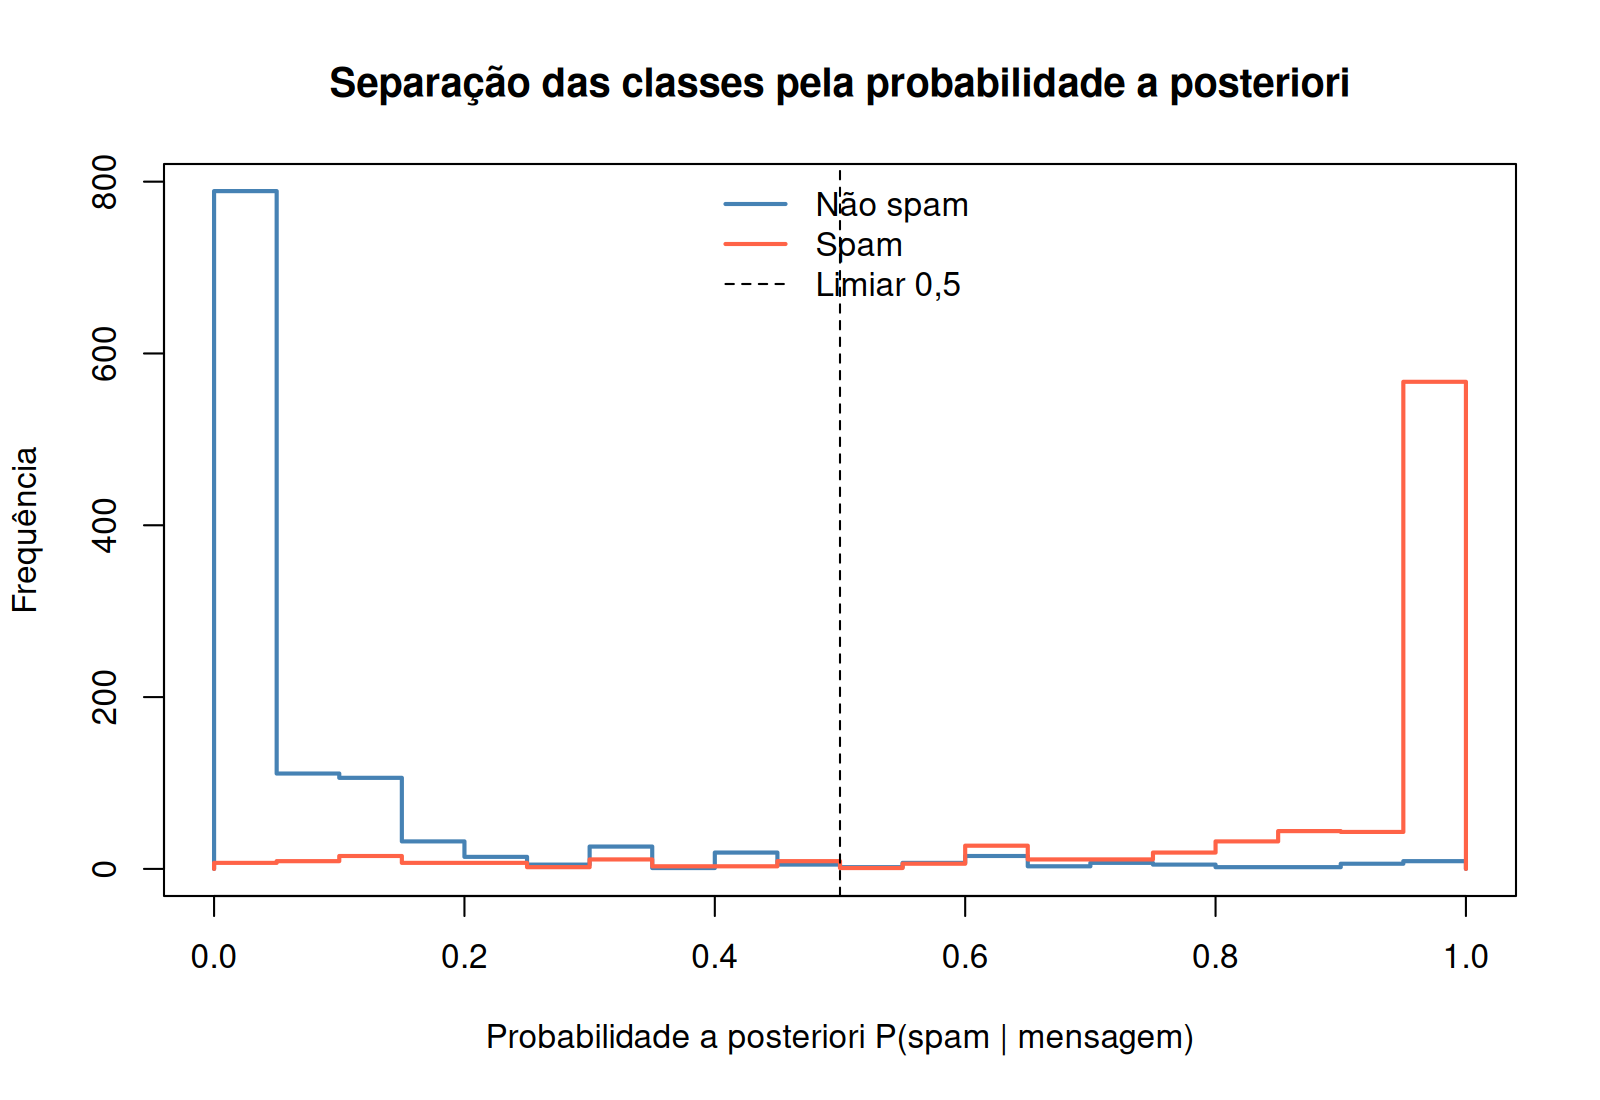
\includegraphics[width=0.8\textwidth]{secoes/07_atividade_integradora/atv_1/imagens/fig_spam_posterior.png}
	\caption{Distribuição da probabilidade a posteriori por classe real.}
	\label{fig:spam_posterior}
\end{figure}

A escolha do limiar envolve um equilíbrio entre os dois tipos de erro. Em um
filtro de spam, o falso positivo costuma ser mais grave que o falso negativo,
pois descarta uma mensagem legítima \cite{sahami1998bayesian}. A
Figura~\ref{fig:spam_limiar} mostra que
elevar o limiar reduz os falsos positivos ao custo de aumentar os falsos
negativos, permitindo ajustar o filtro à tolerância desejada.

\begin{figure}[H]
	\centering
	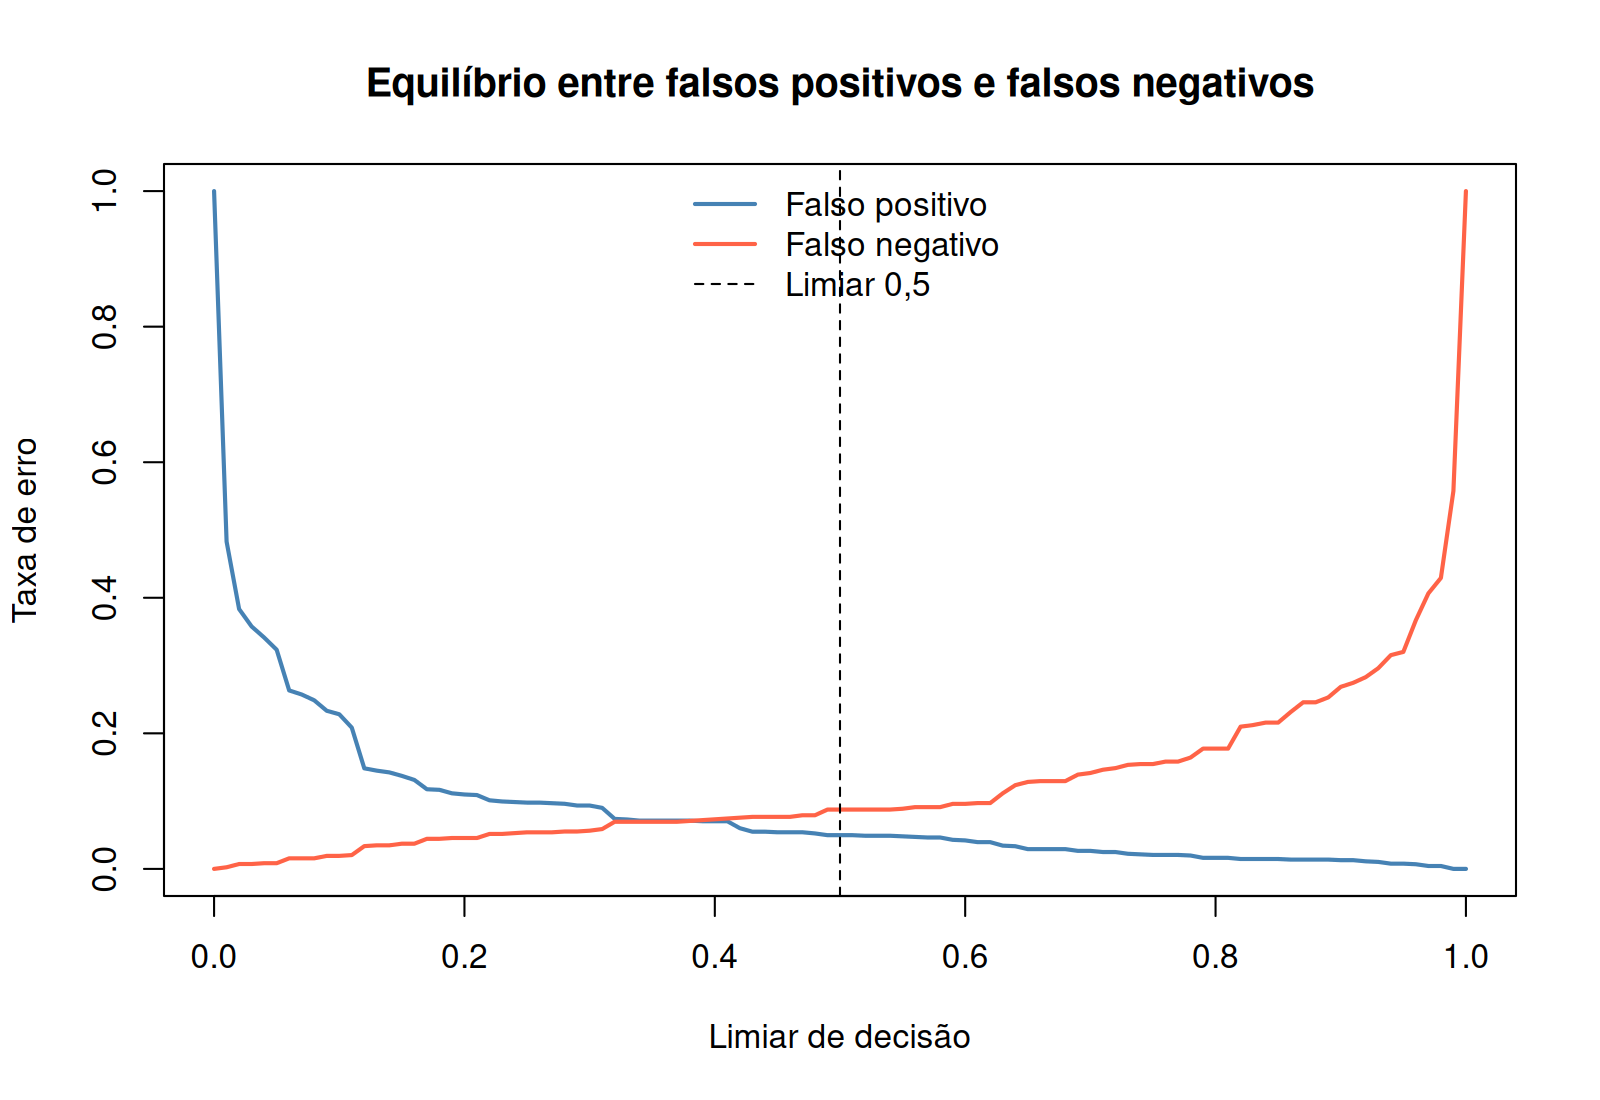
\includegraphics[width=0.8\textwidth]{secoes/07_atividade_integradora/atv_1/imagens/fig_spam_limiar.png}
	\caption{Taxas de falso positivo e falso negativo em função do limiar.}
	\label{fig:spam_limiar}
\end{figure}

A Figura~\ref{fig:spam_sequencial} mostra como a probabilidade de spam é
atualizada palavra a palavra em uma mensagem do conjunto de teste. Ela parte da
priori $0{,}403$, e a presença de palavras típicas de spam eleva a posteriori,
enquanto a ausência de palavras típicas de
não spam também contribui como evidência, de modo que a estimativa final atinge
$0{,}997$.

\begin{figure}[H]
	\centering
	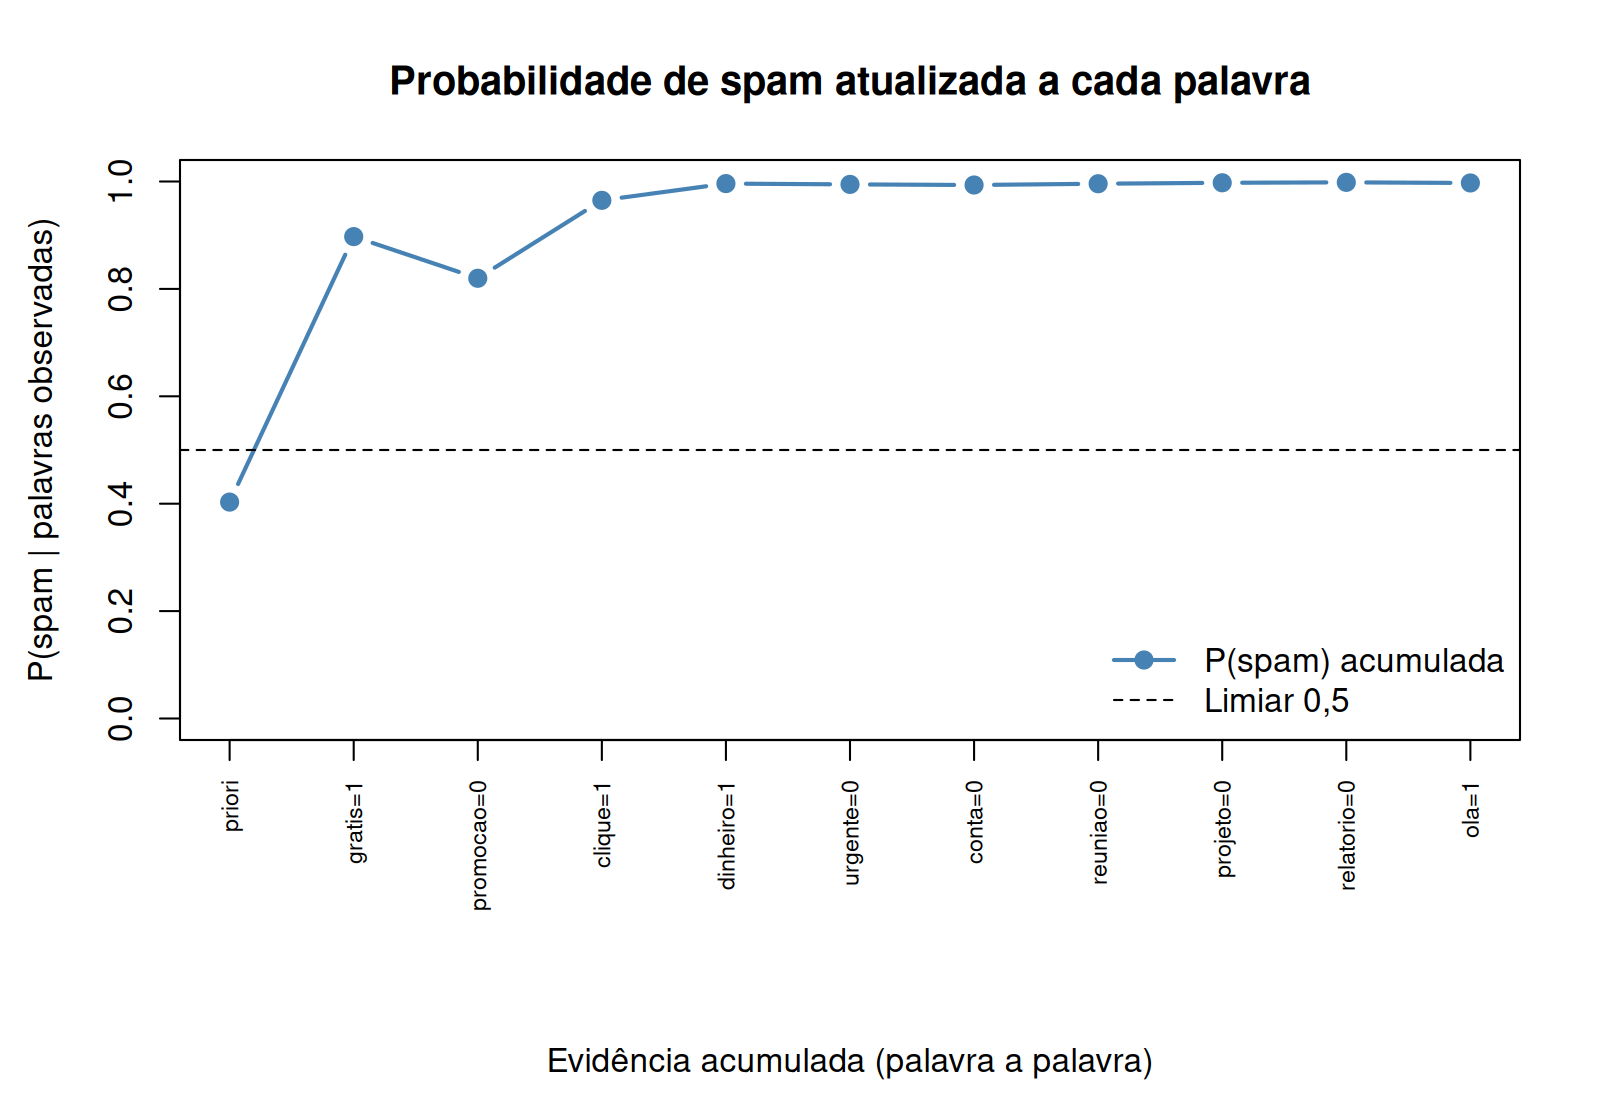
\includegraphics[width=0.8\textwidth]{secoes/07_atividade_integradora/atv_1/imagens/fig_spam_sequencial.png}
	\caption{Atualização da probabilidade a posteriori de spam, palavra a palavra.}
	\label{fig:spam_sequencial}
\end{figure}

A independência condicional vale por construção neste experimento, situação em
que as suposições do modelo são exatamente satisfeitas, o que explica a
proximidade entre as probabilidades estimadas e as teóricas e a alta acurácia. Em
mensagens reais essa hipótese geralmente é violada, pois as palavras apresentam
dependências. Ainda assim, o classificador
ingênuo mantém bom desempenho prático \cite{metsis2006spam}.
